\chapter{従来手法を用いた足動作検知実験}
従来手法の枠組みによって構築した足動作検知のBCIについて説明する。
\section{計測したEEGについて}
まず、被験者が8秒間静止(以後rest状態)と
8秒間足動作(以後walk状態)を8サイクル繰り返したときのEEGを計測した。
被験者はリラックスできる椅子に着席した状態で前方に配置されたディスプレイの
指示に従って動作を行った(図\ref{fig:asibumi})。
ただし、8サイクル中最初の1サイクルについてはフィルタの応答の特性上、
EEGの解析には適さないと判断し、解析時には除外した。
従って以後の解析で用いられるのは7サイクル分のEEGである。
EEGの計測機器としてはg.tec社のg.USBamp(図\ref{fig:usbamp})を用い、ウェット式の電極を採用した。
ウェット式では頭皮と電極の間に導電性のジェルを注入することでEEGを計測する。
EEGの計測時にはジェルの注入を行いながら、すべての電極に関して電極インピーダンスが\(5k\Omega\)
以下になったことを確認した。
またサンプリング周波数は128Hzとした。
\begin{figure}
    \centering
    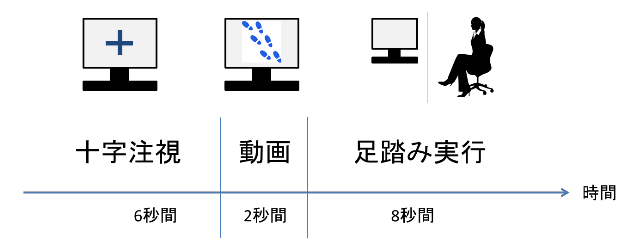
\includegraphics[width=13cm]{images/asibumi.png}
    \caption{EEG計測時のタイムスケジュール}
    \label{fig:asibumi}
\end{figure}
\begin{figure}
    \centering
    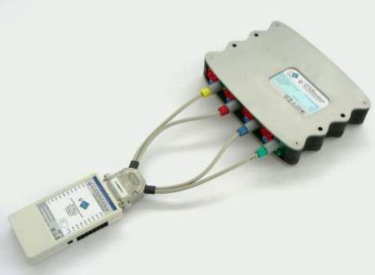
\includegraphics[width=8cm]{images/usbamp.png}
    \caption{g.tec社のg.USBamp}
    \label{fig:usbamp}
\end{figure}

計測に用いた電極の個数は5つであり、Cz、C1、C2、CPz、FCz電極である。
Cz電極は足に関する運動野が脳の頭頂部に存在するため選出し、
スモールラプラシアンフィルタが適用できるように残りの4つを選出した(図\ref{fig:smalllap})。
また、EEGの計測時には定常成分とERDとは無関係な高周波成分を削除するために
通過帯域を0.3Hzから32Hzとした2次のバタワースバンドパスフィルタを用いた。

\section{EEGの解析}
\subsection{ERDの確認}
まずCz電極で計測されたEEGと
Cz電極に対してスモールラプラシアンフィルタを用いた際の
EEGを図\ref{fig:eegsub1}に添付する。
Cz電極に対してスモールラプラシアンフィルタを用いた際の波形\(z(t)\)はである。
\begin{equation}
    z(t) = x_{Cz}(t) - \frac{1}{4}(x_{C1}(t) + x_{C2}(t) + x_{FCz}(t) + x_{CPz}(t))
\end{equation}
ここに\(x_{A}(t)\)はA電極によって計測された波形である。
スモールラプラシアンフィルタの定義から、
頭皮上でCz電極に際立った電位分布が獲得されていることが期待できるが、
図\ref{fig:eegsub1}からその効果を直接確認することは困難である。

\begin{figure}
    \centering
    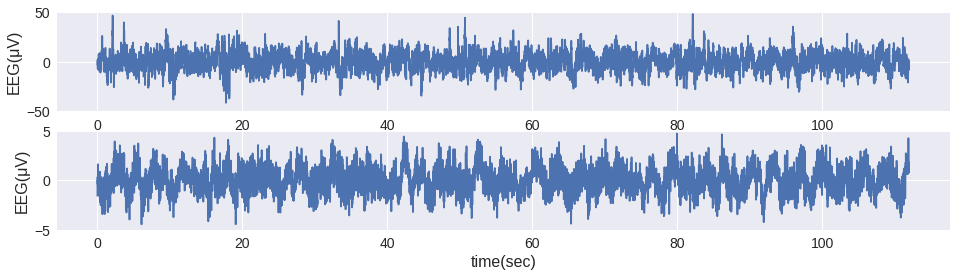
\includegraphics[width=13cm]{images/eeg_sub1.png}
    \caption{Cz電極のEEG(上)とスモールラプラシアンフィルタを用いたEEG(下)}
    \label{fig:eegsub1}
\end{figure}
% \begin{figure}
%     \centering
%     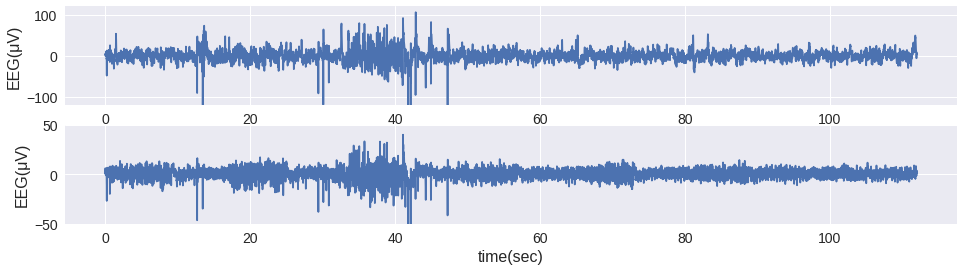
\includegraphics[width=13cm]{images/eeg_sub2.png}
%     \caption{被験者2のCz電極のEEG(上)とスモールラプラシアンフィルタを用いたEEG(下)}
%     \label{fig:eegsub2}
% \end{figure}

% 続いて、PCAとICAによる空間フィルタの設計を試みた。
% それぞれのフィルタから得られる各被験者のEEGの波形を図\ref{fig:bss1}と図\ref{fig:bss2}に示す。
% が\label{section:BSS}にて述べた問題のために、
% 得られた信号のいずれが重要であるかの判断を行うことができなかった。

次にスモールラプラシアンフィルタを用いたEEGの
rest状態(8秒間)の波形とwalk状態(8秒間)の波形それぞれに対してパワースペクトル密度推定を行った。
スペクトル密度推定には1秒間(128点)の時間窓を用いたウェルチのオーバラップ法を利用し、
オーバラップは0.5秒(64点)とした。
rest状態とwalk状態は計7回繰り返し行なっているため図\ref{fig:allERDs}に
7回分すべてのスペクトル密度の比較を示す。
また図\ref{fig:walkERD}に7回分の平均を示す。
ERDの生ずる周波数帯域は個人差があるとされるが、
\(\mu\)律動(8-12Hz)や\(\beta\)律動(18-26Hz)で
パワーの減少が観測できる報告があり\cite{erdfreq}、また\cite{Beta波によるBCI}では
6-40Hzの領域に渡ってERDを検知しBCIを構築した例がある。
概ね先行研究において観測されている周波数帯域でwalk時のパワーの減少が確認された。
\begin{figure}
    \centering
    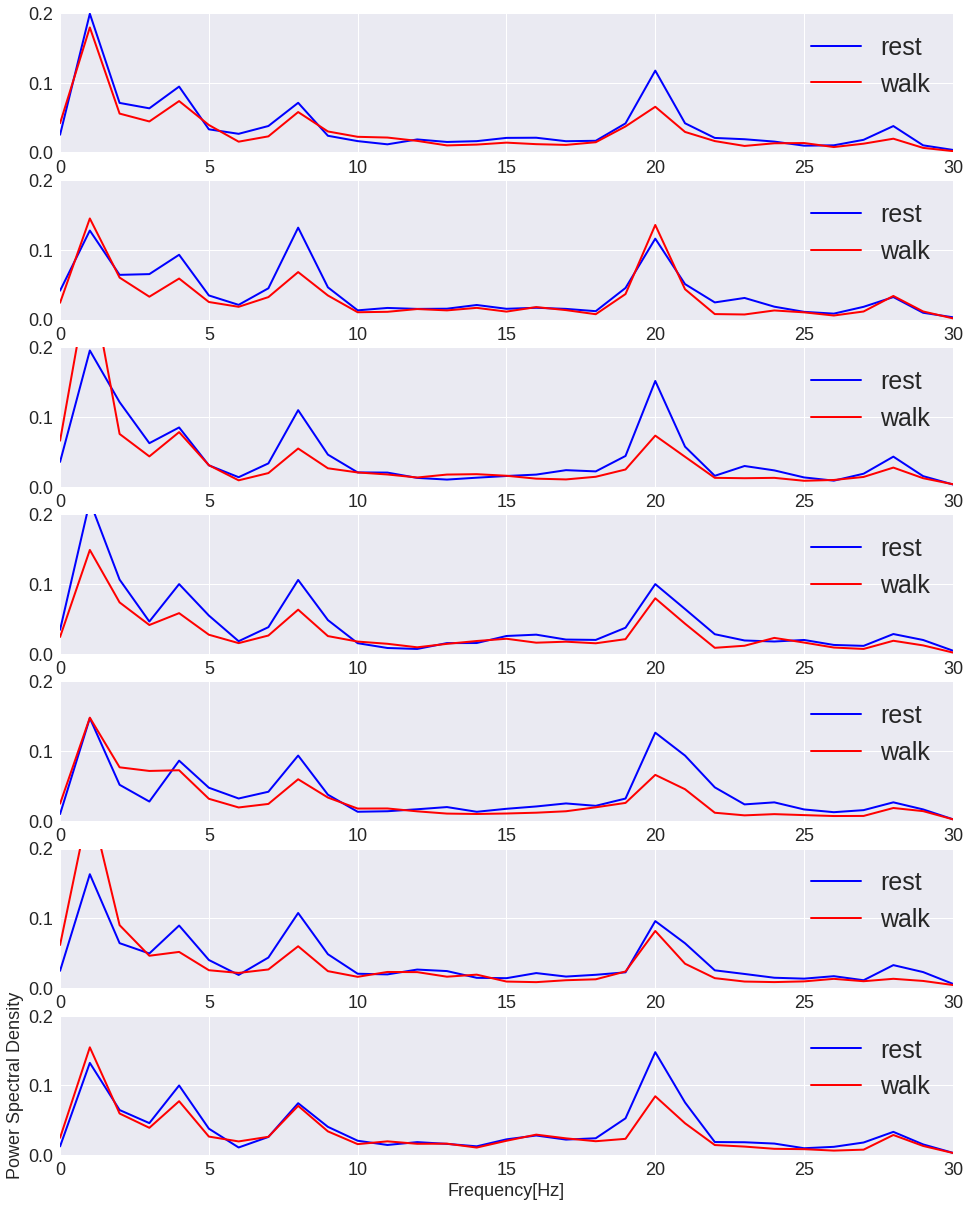
\includegraphics[width=13cm]{images/allERDs}
    \caption{rest時とwalk時のパワースペクトル密度の比較}
    \label{fig:allERDs}
\end{figure}
\begin{figure}
    \centering
    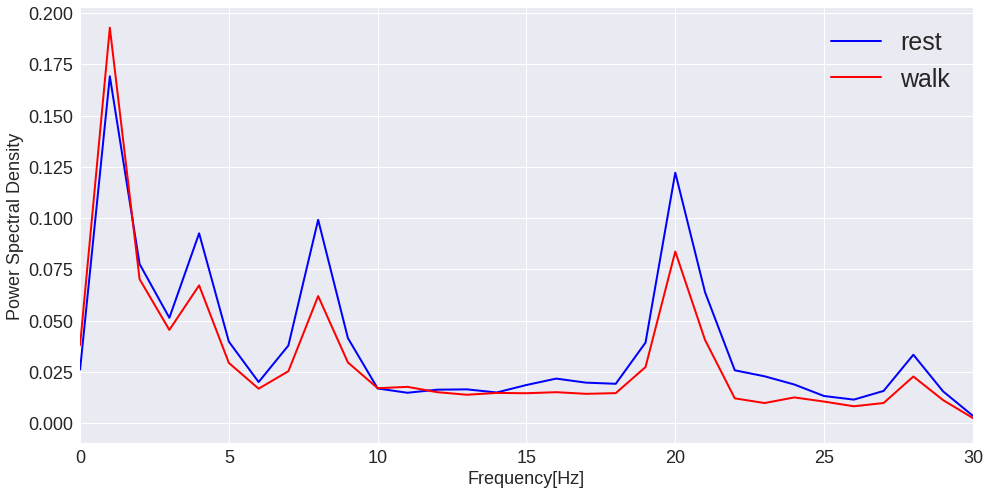
\includegraphics[width=13cm]{images/walkERD}
    \caption{rest時とwalk時のパワースペクトル密度の平均(7回分)の比較}
    \label{fig:walkERD}
\end{figure}

しかし、平均(図\ref{fig:walkERD})を確認すると4、8、20Hz付近で際立ったパワーの減少が見られるが、
個々のスペクトル密度(図\ref{fig:allERDs})は必ずしもパワーの減少が
すべてのサイクルで確認できることを示してはいない。
このことはある一つの周波数帯域のみに着目した場合には
足動作検知の手掛かりを見逃す可能性があることが想定される。

\subsection{時間周波数解析}
